\begin{frame}
\frametitle{Stratégie de recherche}
\begin{small}
\begin{maliste}
\item \'Equipe : David Calvet, Daniela Paredes, Lo\"ic Valery, Dorian Simon, ...
%\vspace*{0.1cm}
%\item \textcolor{magenta}{JHEP 10 (2015) 150}
\vspace*{0.1cm}
\item Processus 4 tops considérés : \textcolor{blue}{non-r\'esonant, r\'esonant, mod\`ele standard}
\end{maliste}
\end{small}

\begin{varblock}[11cm]{Contexte}
\begin{columns}
\begin{column}{0.6\textwidth}
\begin{itemize}
\item Groupe d'analyse : ``same-sign dilepton''
\item Signaux considérés : 
\begin{itemize}
\item[$\rightarrow$] sgluon, VLQ, tt, b', T5/3, ...
\end{itemize}
\end{itemize}
\end{column}
\begin{column}{0.4\textwidth}
%\hspace*{-1.5cm}
%\includegraphics[width=0.6\textwidth]{Figures/FourTops/4topsSMfeynSnapshot.png}
\includegraphics[width=0.65\textwidth]{Figures/FourTops/VLQ_feynDiag.png}

\end{column}
\end{columns}
\end{varblock}

\begin{varblock}[11cm]{Signature}
\begin{columns}
\begin{column}{0.5\textwidth}
\hspace*{0.8cm}
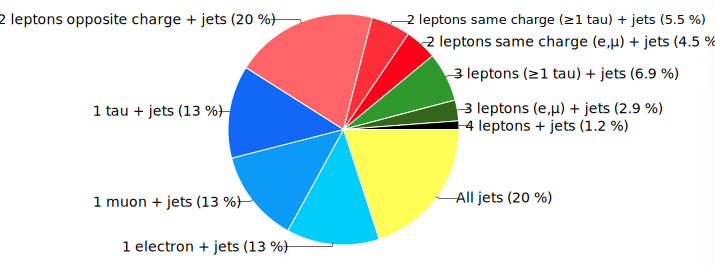
\includegraphics[width=1.2\textwidth]{Figures/FourTops/pie_chart_testinkscape.png}
\end{column}
\hspace*{1.5cm}
\begin{column}{0.5\textwidth}
\begin{maliste}
\item 2 leptons de même charge \\
ou 3 leptons
\item grand nombre de $b$
\item grande $\ETmiss$ 
\item grand $H_T$ 
\end{maliste}
\end{column}
\end{columns}
\end{varblock}
\end{frame}

\begin{frame}
\frametitle{Productions MS et non-résonante}

\begin{maliste}
\item \textcolor{blue}{Production modèle standard}
\begin{columns}
\begin{column}{0.4\textwidth}
\begin{figure}
\begin{center}
\vspace*{-0.5cm}
\hspace*{2cm}
\scalebox{0.65}{
\begin{fmffile}{fgraph-4topsSM}
\begin{fmfgraph*}(110,60)
\fmfleftn{i}{2}\fmfrightn{o}{4}
\fmfset{curly_len}{2mm}
\fmflabel{$g$}{i1}
\fmflabel{$g$}{i2}
\fmflabel{$t$}{o1}
\fmflabel{$\overline{t}$}{o2}
\fmflabel{$t$}{o3}
\fmflabel{$\overline{t}$}{o4}
\fmf{gluon}{i1,v1}
\fmf{fermion}{v1,o1}
\fmf{fermion}{v2,v1}
\fmf{fermion}{o2,v4}
\fmf{gluon}{i2,v3}
\fmf{fermion}{o4,v3}
\fmf{fermion}{v3,v2}
\fmf{fermion}{v4,o3}
\fmf{gluon}{v2,v4}
\fmffixedx{40}{i1,v1}
\fmffixedx{40}{i2,v3}
\end{fmfgraph*}
\end{fmffile}
}
\end{center}
\end{figure}
%\hspace*{0.5cm}
\vspace*{0.1cm}
%\begin{center}
\[\qquad \qquad \quad \quad\sigma\simeq 1~\text{fb \`a }\sqrt{s}=8~\text{TeV}\]
%\end{center}
\end{column}
\begin{column}{0.6\textwidth}
\begin{center}
\vspace*{-0.8cm}
\hspace*{1cm}
\includegraphics[width=0.8\textwidth]{Figures/FourTops/1234topsSMxsec.png}
\end{center}
\end{column}
\end{columns}
\pause
%\vspace*{0.5cm}
\item \textcolor{blue}{Production non-résonante : interaction contact à 4 tops}
\end{maliste}
\begin{columns}
\hspace*{1cm}
\begin{column}{0.6\textwidth}
\[{\cal L} = {\cal L}_\text{SM}+\frac{C}{\Lambda^2}\left(\bar{t}_R\gamma_{ \mu} t_R\right)\left(\bar{t}_R\gamma^{\mu} t_R\right)\]
\begin{itemize}
%\item Interaction contact à 4 tops
%\[{\cal L} = {\cal L}_\text{SM}+\frac{C}{\Lambda^2}\left(\bar{t}_R\gamma_{ \mu} t_R\right)\left(\bar{t}_R\gamma^{\mu} t_R\right)\]
\item Physique BSM avec nouveau vecteur\\
$\rightarrow$ masse $M$\\
$\rightarrow$ limite valable si $M\gtrsim 2$~TeV
\item Pas de contraintes sur $\frac{C}{\Lambda^2}$
\end{itemize}
\end{column}
%\vspace*{0.5cm}
\hspace*{-1cm}
\begin{column}{0.4\textwidth}
\begin{figure}[!htb]
\begin{center}
\scalebox{0.6}{
\begin{fmffile}{fgraph-ContactGluFu1}
\begin{fmfgraph*}(110,60)
\fmfleftn{i}{2}\fmfrightn{o}{4}
\fmfset{curly_len}{2mm}
\fmflabel{$g$}{i1}
\fmflabel{$g$}{i2}
\fmflabel{$t$}{o1}
\fmflabel{$\overline{t}$}{o2}
\fmflabel{$t$}{o3}
\fmflabel{$\overline{t}$}{o4}
\fmf{gluon}{i1,v1}
\fmf{gluon}{i2,v1}
\fmf{gluon,label=$g$}{v1,v2}
\fmf{fermion}{v2,o1}
\fmf{fermion}{v3,v2}
\fmf{fermion}{o2,v3}
\fmf{fermion}{v3,o3}
\fmf{fermion}{o4,v3}
\fmffixedx{20}{i1,v1}
\fmffixedx{20}{i2,v1}
\fmffixed{(25,0)}{v1,v2}
\fmffixed{(25,10)}{v2,v3}
\fmfblob{.07w}{v3}
\end{fmfgraph*} \hspace*{0.8cm}
\end{fmffile}
}
\end{center}
\end{figure}
\begin{figure}[!htb]
\begin{center}
\scalebox{0.6}{
\begin{fmffile}{fgraph-ContactGluFu2}
\begin{fmfgraph*}(110,60)
\fmfleftn{i}{2}\fmfrightn{o}{4}
\fmfset{curly_len}{2mm}
\fmflabel{$g$}{i1}
\fmflabel{$g$}{i2}
\fmflabel{$t$}{o1}
\fmflabel{$\overline{t}$}{o2}
\fmflabel{$t$}{o3}
\fmflabel{$\overline{t}$}{o4}
\fmf{gluon}{i1,v1}
\fmf{fermion}{v1,o1}
\fmf{fermion}{v2,v1}
\fmf{fermion}{o2,v2}
\fmf{gluon}{i2,v3}
\fmf{fermion}{o4,v3}
\fmf{fermion}{v3,v2}
\fmf{fermion}{v2,o3}
\fmffixedx{40}{i1,v1}
\fmffixedx{40}{i2,v3}
\fmfblob{.07w}{v2}
\end{fmfgraph*}
\end{fmffile}
}
\end{center}
\end{figure}
\end{column}
\end{columns}

\end{frame}

\begin{frame}
\frametitle{Production effective : interaction de contact}
\begin{center}
Exemples de modèles conduisant à une interaction de contact
\end{center}
\begin{columns}
\begin{column}{0.5\textwidth}
\begin{block}{\center Top composite (arXiv:0712.3057,1010.6340,...)}
\vspace*{0.2cm}
\begin{figure}
\begin{center}
\scalebox{0.65}{
\begin{fmffile}{fgraph-TopComposite}
\begin{fmfgraph*}(110,60)
\fmfleftn{i}{2}\fmfrightn{o}{4}
\fmfset{curly_len}{2mm}
\fmflabel{$g$}{i1}
\fmflabel{$g$}{i2}
\fmflabel{$t$}{o1}
\fmflabel{$\overline{t}$}{o2}
\fmflabel{$t$}{o3}
\fmflabel{$\overline{t}$}{o4}
\fmf{gluon}{i1,v1}
\fmf{fermion}{v1,o1}
\fmf{fermion}{v2,v1}
\fmf{fermion}{o2,v4}
\fmf{gluon}{i2,v3}
\fmf{fermion}{o4,v3}
\fmf{fermion}{v3,v2}
\fmf{fermion}{v4,o3}
\fmf{photon,label=$\rho$}{v2,v4}
\fmffixedx{40}{i1,v1}
\fmffixedx{40}{i2,v3}
\end{fmfgraph*}
\end{fmffile}
}
\end{center}
\end{figure}
\vspace*{-0.3cm}
\begin{figure}[!htb]
\begin{center}
%\includegraphics[width=0.75\textwidth]{Figures/FourTops/TopCompositeXsecJingShuEtAl.png}
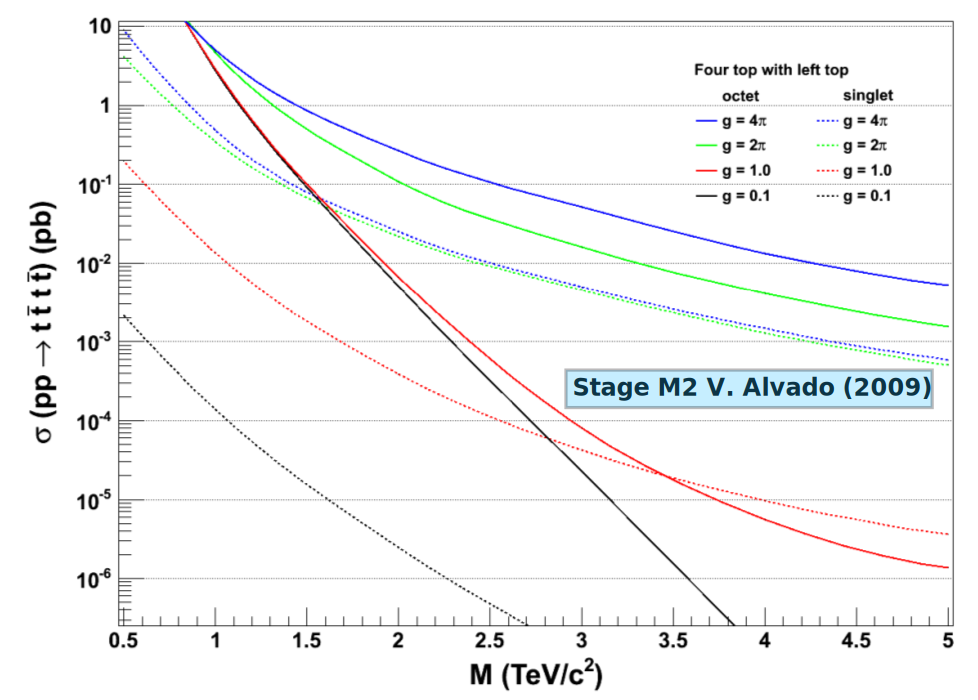
\includegraphics[width=0.95\textwidth]{Figures/FourTops/PlotVincentAlvado.png}
\put(-40,35){\tiny{$\sqrt{s}=14~$TeV}}
\end{center}
\end{figure}

\end{block}
\pause
\end{column}
\begin{column}{0.55\textwidth}
\begin{block}{\center RS modifié $t\bar{t} g_{KK}$ (arXiv:0710.2234)}
\begin{itemize}
\item Champs standards dans bulk
\item Higgs sur TeV brane
\item Couplage fort entre $g_{KK}$ et $t_R$
%\item Couplage $ggg_{KK}$ supprimé (profiles $\perp$)
%\item Processus favorisé : $gg(q\bar{q})\rightarrow t_R \bar{t}_R g_{KK}$
\end{itemize}

\begin{figure}
\begin{center}
\scalebox{0.65}{
\begin{fmffile}{fgraph-ttbargKKproduction}
\begin{fmfgraph*}(110,60)
\fmfleftn{i}{2}\fmfrightn{o}{3}
\fmfset{curly_len}{2mm}
\fmflabel{$g$}{i1}
\fmflabel{$g$}{i2}
\fmflabel{$t$}{o1}
\fmflabel{$\overline{t}$}{o2}
\fmflabel{$g_{KK}$}{o3}
\fmf{gluon}{i1,v1}
\fmf{gluon}{v1,i2}
\fmf{gluon,label=$g$}{v1,v2}
\fmf{fermion}{v2,o1}
\fmf{fermion}{v3,v2}
\fmf{fermion}{o2,v3}
\fmf{gluon}{v3,o3}
\fmffixedx{25}{i1,v1}
\fmffixedx{25}{i2,v1}
\fmffixed{(20,0)}{v1,v2}
%\fmffixed{(30,10)}{v2,v3}
\end{fmfgraph*} 
\end{fmffile}
}
\end{center}
\end{figure}
\vspace*{0.2cm}

\end{block}
\pause
\begin{block}{Z' \english{top-philic} (arXiv:0912.0004)}
\begin{itemize}
\item $SU(3)_C\times SU(2)_L\times U(1)_Y \times U(1)'$\\
$\rightarrow Z'$ et $\nu'$ (candidat DM)
\item Processus favorisé : $gg(q\bar{q})\rightarrow t_R \bar{t}_R Z'$
%\item Couplage fort $Z'tt_R$
\end{itemize}
\end{block}
\end{column}
\end{columns}
\end{frame}

\begin{frame}
\frametitle{Production résonante : modèle 2UED/RPP}

\begin{textblock*}{5cm}(.95\textwidth,0.4cm)%
  \scriptsize{ 
    \textcolor{white}{arXiv:0907.4993}\\
    \textcolor{white}{arXiv:1104.3800}\\
    \textcolor{white}{arXiv:1107.4616}\\
    arXiv:1209.6556\\
    arXiv:1210.0384\\
    arXiv:1302.4750
  }
\end{textblock*}

\MyTextNoTilt{\'Etage : $(k,l)$}
\begin{maliste}
\item Extension ``simple'' du modèle standard :
\begin{itemize}
\item 2 dimensions supplémentaires universelles
\item Compactification : Real Projective Plane (RPP)
\end{itemize} 
\vspace*{0.1cm}
\item Intérêt : candidat matière noire (photon $A^{\left(1,0\right)}$)
\end{maliste}
\begin{columns}
\begin{column}{0.5\textwidth}
%\vspace*{0.1cm}
\begin{figure}
\includegraphics[width=0.95\textwidth]{Figures/FourTops/cosmoConstraints2UEDRPP_symmetric.png}
\put(-95,88){\scriptsize{JHEP, 1301 : 147, 2013}}
\put(-40,70){\scriptsize{$R_4= R_5$}}
\end{figure}
\vspace*{-1.28cm}
\begin{figure}
\includegraphics[width=0.98\textwidth]{Figures/FourTops/cosmoConstraints2UEDRPP.png}
\put(-40,25){\scriptsize{$R_4\neq R_5$}}
\end{figure}
\end{column}
\hspace*{-0.3cm}
\begin{column}{0.55\textwidth}
\begin{block}{Paramètres}
\begin{maliste}
\item Rayons : $R_4$, $R_5$
\[
\begin{pmatrix}
R_4 \\
R_5
\end{pmatrix}
\Rightarrow
\begin{pmatrix}
\xi=\frac{R_4}{R_5} \\
m_\text{KK}=\frac{1}{R_4}
\end{pmatrix}
\]
\vspace*{0.1cm}
\item Cut-off : $\Lambda$
\item Rapport embranchement : $A^{(1,1)}\rightarrow t\bar{t}$
\end{maliste}
\end{block}
\begin{block}{Contraintes cosmologiques}
\begin{maliste}
\item $\xi=1$ défavorisé
\item $m_\text{KK}\in\left[700;1000\right]$~GeV 
\end{maliste}
\end{block}
\end{column}
\end{columns}
\end{frame}

\begin{frame}
\frametitle{2UED/RPP : phénoménologie au LHC}
\begin{maliste}
\item Phénoménologie riche : contributions étages $(1,0)$, $(1,1)$ et $(2,0)$
\item Contraintes à partir des étages $(1,0)$, $(2,0)$ : $m_\text{KK}\gtrsim 600~$GeV %(arXiv:1209.6556,arXiv:1302.4750)
\item \textcolor{magenta}{\'Etages $(1,1)$ et $(2,0)$ : événements 4 tops}

\vspace*{0.3cm}
\begin{figure}
\begin{center}
\scalebox{0.55}{
\begin{fmffile}{fgraph-2UEDRPP}
\unitlength = 0.45mm

\begin{fmfgraph*}(160,90)

%\fmfpen{thick}                                                                                       
\fmfleft{i2,i1}
\fmfright{t1,t2,t3,t4}
\fmftop{i1,p1,p2,a5,a6,a7,t4}
\fmfbottom{i2,p3,a1,a2,a3,a4,t1}
\fmfset{curly_len}{2mm}
\fmf{fermion,tension=1}{i1,v1}
\fmf{fermion,tension=.2}{v8,a5}
\fmf{fermion,tension=.2}{a6,v9}
\fmf{fermion,tension=.2}{v10,a7}
\fmf{fermion,tension=.5}{t3,v11,t4}
\fmf{fermion,tension=.2}{a1,v3}
\fmf{fermion,tension=.2}{v4,a2}
\fmf{fermion,tension=.2}{a3,v5}
\fmf{fermion,tension=.2}{v6,a4}
\fmf{fermion,tension=.5}{t1,v7,t2}

\fmf{gluon,tension=1}{i2,v2}


\fmf{gluon,label=${\scriptstyle g}^{\scriptscriptstyle (1,,1)}\;\;$}{v1,v2}
\fmf{gluon,tension=1.2}{v2,v3}
\put(37,33){${\scriptstyle g}^{\scriptscriptstyle (1,1)}$}

\fmf{boson,label=${\scriptstyle W}^{\scriptscriptstyle +(1,,1)}$}{v8,v9}
\fmf{boson,label=${\scriptstyle Z}^{\scriptscriptstyle (1,,1)}$,l.s=left}{v4,v5}
\fmf{boson,tension=0.6}{v6,v7}
\put(120,20){${\scriptstyle A}^{\scriptscriptstyle (1,1)}$}

\fmf{boson,tension=0.6}{v10,v11}
\put(115,62){${\scriptstyle A}^{\scriptscriptstyle (1,1)}$}

\fmf{fermion,tension=1.2,label=${\scriptstyle u_L}^{\scriptscriptstyle (1,,1)}$}{v1,v8}
\fmf{fermion,label=${\scriptstyle \nu_\tau}^{\scriptscriptstyle (1,,1)}$,l.s=right}{v9,v10}
\fmf{fermion,label=$\;\;{\scriptstyle c_{L}}^{\scriptscriptstyle (1,,1)}$,l.s=left}{v3,v4}
\fmf{fermion,label=$\;\;{\scriptstyle \mu}^{\scriptscriptstyle -(1,,1)}\;\;$,l.s=left}{v5,v6}
\fmfblob{.04w}{v11}
\fmfblob{.04w}{v7}
%\fmfv{decor.shape=circle,decor.filled=full,decor.size=10}{v11}                                       
%\fmfv{decor.shape=circle,decor.filled=full,decor.size=10}{v7}   

\fmflabel{$u$}{i1}
\fmflabel{$g$}{i2}
\fmflabel{\textcolor{blue}{$\bar{c}$}}{a1}
\fmflabel{\textcolor{blue}{$c$}}{a2}
\fmflabel{\textcolor{blue}{$\mu^+$}}{a3}
\fmflabel{\textcolor{blue}{$\mu^{-}$}}{a4}
\fmflabel{\textcolor{blue}{$d$}}{a5}
\fmflabel{\textcolor{blue}{$\tau^+$}}{a6}
\fmflabel{\textcolor{blue}{$\nu_\tau$}}{a7}
\fmflabel{\textcolor{red}{$\bar{t}$}}{t1}
\fmflabel{\textcolor{red}{$t$}}{t2}
\fmflabel{\textcolor{red}{$\bar{t}$}}{t3}
\fmflabel{\textcolor{red}{$t$}}{t4}

\end{fmfgraph*}
\hspace*{1cm}
\begin{fmfgraph*}(150,80)

%\fmfpen{thick}                                                                                       

\fmfleft{i2,i1}
\fmfright{u1,t1,t2,t3,t4,u2}
\fmfset{curly_len}{2mm}

\fmf{gluon,tension=2}{i1,v1}
\fmf{gluon,tension=2}{i2,v2}
\fmf{fermion}{u1,a1}
\fmf{fermion,tension=2,label=${\scriptstyle \bar{u}_R^{\scriptscriptstyle (1,,1)}}$}{a1,v2}
\fmf{fermion,label=${\scriptstyle u_R^{\scriptscriptstyle (1,,1)}}$}{v2,v1}
\fmf{fermion,tension=2,label=${\scriptstyle u_R^{\scriptscriptstyle (1,,1)}}$}{v1,a2}
\fmf{fermion}{a2,u2}
\fmf{boson,label=${\scriptstyle A^{\scriptscriptstyle (1,,1)}}$}{a1,b1}
\fmf{boson,label=${\scriptstyle A^{\scriptscriptstyle (1,,1)}}$,l.s=right}{a2,b2}
\fmf{fermion,tension=0.8}{t1,b1}
\fmf{fermion,tension=0.5}{b1,t2}
\fmf{fermion,tension=0.8}{t3,b2}
\fmf{fermion,tension=0.5}{b2,t4}

\fmfblob{.04w}{b1}
\fmfblob{.04w}{b2}
%\fmfv{decor.shape=circle,decor.filled=full,decor.size=10}{b1}                                        
%\fmfv{decor.shape=circle,decor.filled=full,decor.size=10}{b2}  
\fmflabel{$g$}{i1}
\fmflabel{$g$}{i2}
\fmflabel{\textcolor{blue}{$\bar{u}$}}{u1}
\fmflabel{\textcolor{blue}{$u$}}{u2}
\fmflabel{\textcolor{red}{$\bar{t}$}}{t1}
\fmflabel{\textcolor{red}{$t$}}{t2}
\fmflabel{\textcolor{red}{$\bar{t}$}}{t3}
\fmflabel{\textcolor{red}{$t$}}{t4}
\end{fmfgraph*}
\end{fmffile}
}
\end{center}
\end{figure}
\end{maliste}

\begin{columns}
\begin{column}{0.6\textwidth}
\begin{figure}[!htb]
\begin{center}
%\hspace*{-1cm}
\includegraphics[width=0.85\textwidth]{Figures/FourTops/Xsec2UEDRPPVsMkk.png}
\put(-55,85){\scriptsize{$\sqrt{s}=8~$TeV}}
\end{center}
\end{figure}
\end{column}
\begin{column}{0.45\textwidth}
\begin{maliste}
\item Accessible au LHC $8$~TeV\\
$\Rightarrow$ Possibilité d'améliorer les contraintes existantes
\end{maliste}
\end{column}
\end{columns}

\end{frame}

\begin{comment}
\begin{frame}
\frametitle{Simulation}

\begin{small}
\begin{maliste}
\item Interaction de contact : 
\begin{itemize}
\item MadGraph5 + Pythia8
\item Cinématique indépendante de $C/\Lambda^2$ $\rightarrow$ un seul échantillon 
\item Nouveau vecteur : $M = 100~$TeV
\end{itemize}
\vspace*{0.3cm}
\item 2UED/RPP : 
\begin{itemize}
\item MadGraph5 + BRIDGE + Pythia8
\item Masses particules étage $(1,1)$ au NLO
\item Valeurs paramètres : $\xi=1$, $m_\text{KK}=600,800,1000,1200$~GeV
\end{itemize}
\end{maliste}
\end{small}

%Sur plot ci-dessous, rajouter distribution 4 tops SM

\vspace*{-0.5cm}
\begin{figure}[!htb]
\begin{center}
%\hspace*{-1cm}
\includegraphics[width=0.55\textwidth]{Figures/FourTops/EnergyTop.png}
\includegraphics[width=0.55\textwidth]{Figures/FourTops/NoAccompanyingQuarks.png}
\end{center}
\end{figure}

\end{frame}
\end{comment}

